\documentclass{standalone}
    \usepackage{tikz}
    \begin{document}
      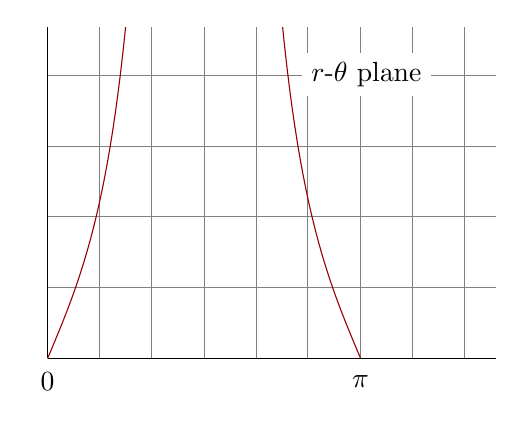
\begin{tikzpicture}[x=12,scale=3]
        \clip (-0.2,-0.2) rectangle (4.5,1.4);
      \draw[->] (0,0) -- (6.28,0) node[right] {$\theta$};
      \draw[->] (0,0) -- (0,1.5) node[above] {$r$};
      \foreach \x in {0.52, 1.04, 1.57, 2.09, 2.61, 3.14, 3.66, 
                     4.18, 4.71, 5.23, 5.75, 6.28}
        \draw[gray,very thin] (\x,0)--(\x,1.5);
      \foreach \x in {0.3, 0.6, 0.9,1.2}
        \draw[gray,very thin] (0,\x)--(6.28,\x);
        \draw(3.14,-0.1) node {$\pi$};
        \draw(0,-0.1) node {$0$};
        \draw[red!60!black,domain=0:0.9,samples=1000] plot 
            (\x, {sin((\x)r)/cos((\x)r)/cos((\x)r)});
        \draw[red!60!black,domain=2.24:3.14,samples=1000] plot 
            (\x, {sin((\x)r)/cos((\x)r)/cos((\x)r)});
         \draw (3.2,1.2) node [fill=white]
            {$r$-$\theta$ plane};
      \end{tikzpicture}
    \end{document}